\documentclass[10pt,twocolumn,letterpaper]{article}
\usepackage{authblk}

%%%%%%%%% PAPER TYPE  - PLEASE UPDATE FOR FINAL VERSION
% \usepackage[review]{cvpr}      % To produce the REVIEW version
\usepackage{cvpr}              % To produce the CAMERA-READY version
%\usepackage[pagenumbers]{cvpr} % To force page numbers, e.g. for an arXiv version
\usepackage[T1]{fontenc}
\usepackage[utf8]{inputenc}

% Include other packages here, before hyperref.
\usepackage{graphicx}
\usepackage{amsmath}
\usepackage{amssymb}
\usepackage{booktabs}
\usepackage[shortlabels]{enumitem}
% It is strongly recommended to use hyperref, especially for the review version.
% hyperref with option pagebackref eases the reviewers' job.
% Please disable hyperref *only* if you encounter grave issues, e.g. with the
% file validation for the camera-ready version.
%
% If you comment hyperref and then uncomment it, you should delete
% ReviewTempalte.aux before re-running LaTeX.
% (Or just hit 'q' on the first LaTeX run, let it finish, and you
%  should be clear).
\usepackage[pagebackref,breaklinks,colorlinks]{hyperref}


% Support for easy cross-referencing
\usepackage[capitalize]{cleveref}
\crefname{section}{Sec.}{Secs.}
\Crefname{section}{Section}{Sections}
\Crefname{table}{Table}{Tables}
\crefname{table}{Tab.}{Tabs.}


%%%%%%%%% PAPER ID  - PLEASE UPDATE
\def\cvprPaperID{*****} % *** Enter the CVPR Paper ID here
\def\confName{CVPR}
\def\confYear{2023}


\begin{document}

%%%%%%%%% TITLE - PLEASE UPDATE
\title{NTIRE 2023 Efficient SR Challenge Factsheet\\-Efficient Deep Residual Network-}
\author{Zhao Zhang, Baiang Li, Huan Zheng, Suiyi Zhao, Yangcheng Gao, Jiahuan Ren\\
Hefei University of Technology\\
Hefei, China\\
{\tt\small cszzhang@gmail.com, ztmotalee@gmail.com,  huanzheng1998@gmail.com, meranderzhao@gmail.com, gaoyangcheng576@gmail.com, hmzry10086@outlook.com}
% For a paper whose authors are all at the same institution,
% omit the following lines up until the closing ``}''.
% Additional authors and addresses can be added with ``\and'',
% just like the second author.
% To save space, use either the email address or home page, not both
%Baiang Li, HuanZheng, Suiyi Zhao, Yangcheng Gao, Jiahuan Ren

}
% {Hefei University of Technology\\Hefei, China}
\maketitle
\section{Introduction}

This factsheet template is meant to structure the description of the contributions made by each participating team in the NTIRE 2023 challenge on efficient image super-resolution. 

Ideally, all the aspects enumerated below should be addressed.
The provided information, the codes/executables and the achieved performance on the testing data are used to decide the awardees of the NTIRE 2023 challenge. 

Reproducibility is a must and needs to be checked for the final test results in order to qualify for the NTIRE awards. 

The main winners will be decided based on overall performance and a number of awards will go to novel, interesting solutions and to solutions that stand up as the best in a particular subcategory the judging committee will decided. Please check the competition webpage and forums for more details.

The winners, the awardees and the top ranking teams will be invited to co-author the NTIRE 2023 challenge report and to submit papers with their solutions to the NTIRE 2023 workshop. Detailed descriptions are much appreciated.

The factsheet, \href{https://github.com/ofsoundof/NTIRE2023_ESR}{source codes/executables}, trained models should be sent to \textbf{all of the NTIRE 2023 challenge organizers (Yawei Li, Yulun Zhang, and Radu Timofte)} by email.


\section{Email final submission guide}

\noindent To: {yawei.li@vision.ee.ethz.ch} \\ {yulun100@gmail.com} \\ {timofte.radu@gmail.com}\\
\noindent cc: your\_team\_members\\
Title: NTIRE 2023 Efficient SR Challenge - TEAM\_NAME - TEAM\_ID\\

To get your TEAM\_ID, please register at \href{https://docs.google.com/spreadsheets/d/1oekPThh5mq9qKax0hPZiQSHlqTjaoQa-IBfrQkwN7gk/edit?usp=sharing}{Google Sheet}. Please fill in your Team Name, Contact Person, and Contact Email in the first empty row from the top of sheet.
% 
Body contents should include: 

\begin{enumerate}[a)]
\item team name 

\item team leader's name and email address 

\item rest of the team members 

\item user names on NTIRE 2023 CodaLab competitions 

\item Code, pretrained model, and factsheet download command, e.g. \texttt{git clone ...}, \texttt{wget ...}

\item Result download command, e.g. \texttt{wget ...}
\begin{itemize}
    \item Please provide different urls in e) and f)
\end{itemize}
\end{enumerate}



\noindent Factsheet must be a compiled pdf file together with a zip with .tex factsheet source files. Please provide a detailed explanation.


\section{Code Submission}

The code and trained models should be organized according to the \href{https://github.com/ofsoundof/NTIRE2023_ESR}{GitHub repository}. This code repository provides the basis to compare the various methods in the challenge. \textbf{Code scripts based on other repositories will not be accepted.} Specifically, you should follow the steps below.
\begin{enumerate}
    \item Git clone \href{https://github.com/ofsoundof/NTIRE2023_ESR}{the repository.}
    \item Put your model script under the \texttt{models} folder. Name your model script as \texttt{[Your\_Team\_ID]\_[Your\_Model\_Name].py}.
    \item Put your pretrained model under the \texttt{model\_zoo} folder. Name your model checkpoint as \texttt{[Your\_Team\_ID]\_[Your\_Model\_Name].[pth or pt or ckpt]}
    \item Modify \texttt{model\_path} in \texttt{test\_demo.py}. Modify the imported models.
    \item \texttt{python test\_demo.py}
\end{enumerate}
Please send us the command to download your code, e.g. \texttt{git clone [Your repository link]}
When submitting the code, please remove the LR and SR images in \texttt{data} folder to save the bandwidth.

\section{Factsheet Information}

The factsheet should contain the following information. Most importantly, you should describe your method in detail. The training strategy (optimization method, learning rate schedule, and other parameters such as batch size, and patch size) and training data (information about the additional trainning data) should also be explained in detail.

\subsection{Team details}

\begin{itemize}
\item Team name\par
MotaLee
\item Team leader name\par
Zhao Zhang                          
\item Team leader address, phone number, and email \par
9th Floor, Block A, Science And Education Building, Hefei University of Technology (Emerald Lake Campus), 485 Danxia Road, Hefei 230601, China,\par
(+86)18356138079,\par
cszzhang@gmail.com
\item Rest of the team members\par   
Baiang Li, Hefei University of Technology (HFUT)\par
Huan Zheng, Hefei University of Technology (HFUT)\par
Suiyi Zhao, Hefei University of Technology (HFUT)\par
Yangcheng Gao, Hefei University of Technology (HFUT)\par
Jiahuan Ren, Hefei University of Technology (HFUT)
\item Team website URL (if any)                   
\item Affiliation\par
Hefei University of Technology
\item Affiliation of the team and/or team members with NTIRE 2023 sponsors (check the workshop website)
\item User names and entries on the NTIRE 2023 Codalab competitions (development/validation and testing phases)
MotaLee, 2(validation)
\item Best scoring entries of the team during development/validation phase\par
best scoring entry:2, score:28.977731

\item Link to the codes/executables of the solution(s)
\end{itemize}

\subsection{Method details}

You should describe your proposed solution in detail. This part is equivalent to the methodology part of a conference paper submission. The description should cover the following details.
\begin{figure*}[t]
	\centering
	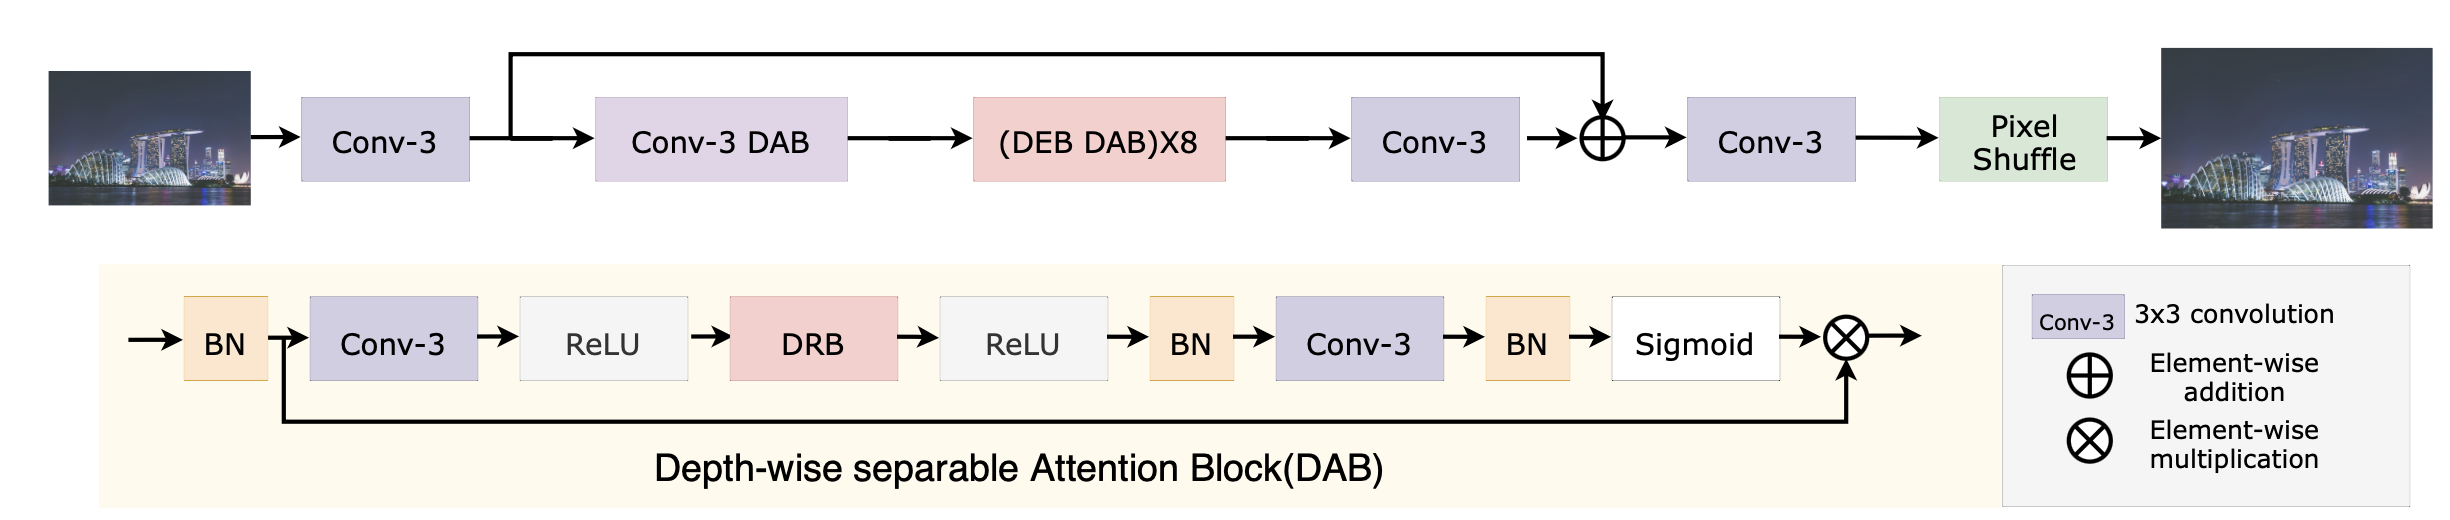
\includegraphics[width=0.9\textwidth]{edrn.png}
	\caption{The structure of the proposed EDRN.}
	\label{Fig.main1}
\end{figure*}

\begin{figure}[!]
	\centering
	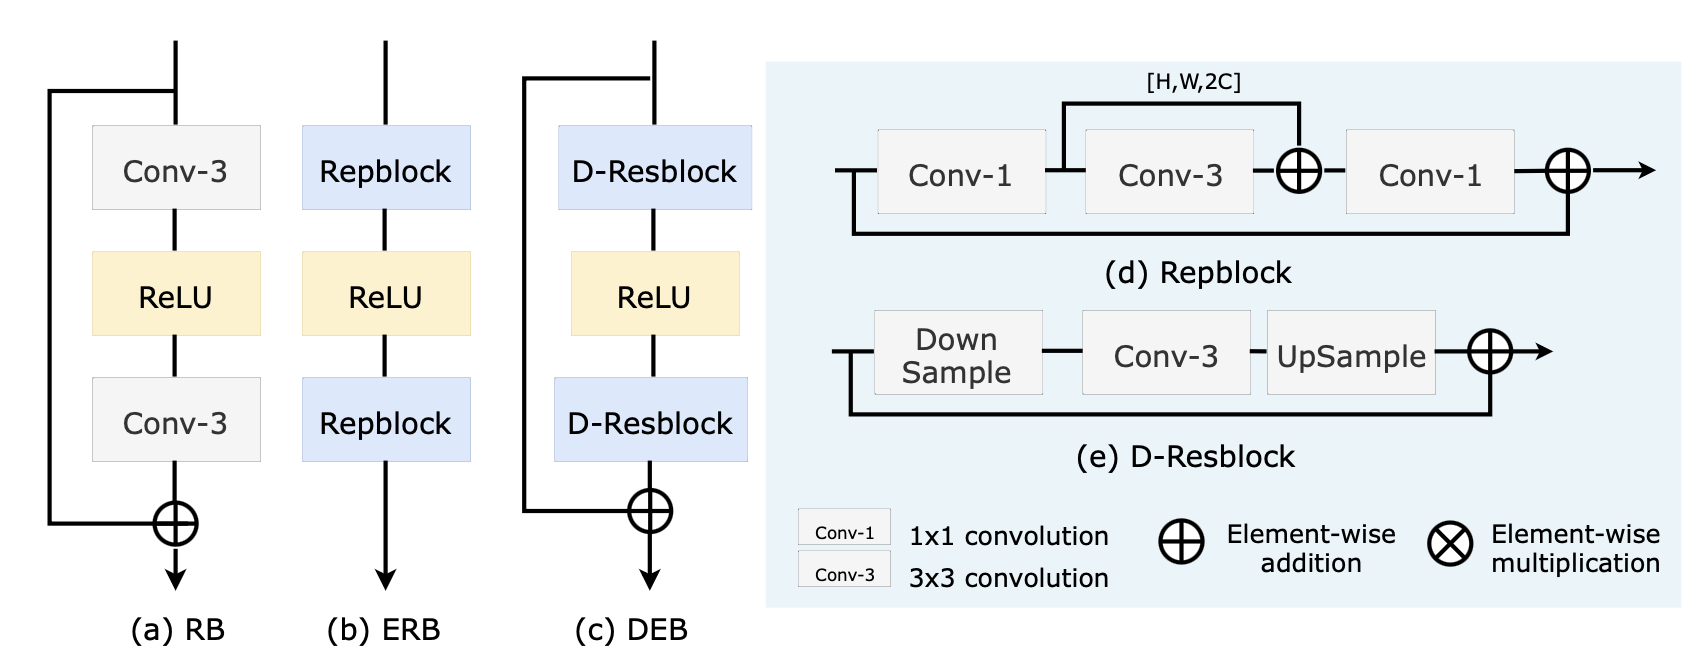
\includegraphics[width=0.5\textwidth]{dab.png}
	\caption{The structure of our proposed DEB and DRB. To show the difference, we show some modules of FMEN.}
	\label{Fig.main}
\end{figure}
\begin{itemize}
\item General method description (How is the network designed.)                                
Considering the requirements of the Efficient Super-Resolution task, we need to improve the performance of the model as much as possible under the limited computational cost. Although FMEN can efficiently extract features while saving time and space memory, it still cannot meet the corresponding accuracy requirements. We infer that this is because it still cannot effectively extract the correlation features between pixels of low-resolution images and Deep connections between different pixels of an image. At the same time, it uses relatively few residual connections in order to reduce computational cost consumption, which will cause it to lose the original features in the process of feature extraction, resulting in reduced accuracy and unable to meet the final competition requirements. Therefore, we design an Efficient Deep Residual Network (EDRN). Specifically, our backbone network is the same as FMEN. At the same time, in order to better extract the deep features of the image, we modified the Repblock, designed a D-Resblock, and used a residual connection to preserve the original features of the image.

\item Training strategy\par
We trained a total of 300 epochs to bring the model to convergence. The number of feature maps of DRB and DAB is set to 64 and 16, respectively. Our initial learning rate is set to $2x10^{-4}$, and the learning rate decays to $4x10^{-5}$ after 200 epochs of epoch. Meanwhile, in the first 250 epochs, we use L1 loss, and in the last 50 epochs we use L2 loss. Our other settings are exactly the same as FMEN.
\item Representative image / diagram / pipeline of the method(s):\par
see Fig \ref{Fig.main1} and Fig \ref{Fig.main}. 
\item Experimental results
\item References                                               
\end{itemize}

Additionally, you can refer to the following items to detail your description.
\begin{itemize}
\item Total method complexity (number of parameters, FLOPs, GPU memory consumption, number of activations, runtime)
\item Which pre-trained or external methods / models have been used (for any stage, if any) 
\item Which additional data has been used in addition to the provided NTIRE training and validation data (at any stage, if any) 
\item Training description
\item Testing description
\item Quantitative and qualitative advantages of the proposed solution
\item Results of the comparison to other approaches (if any)
\item Results on other benchmarks (if any)
\item Novelty degree of the solution and if it has been previously published
\item It is OK if the proposed solution is based on other works (papers, reports, Internet sources (links), etc). It is ethically wrong and a misconduct if you are not properly giving credits and hide this information.
\end{itemize}

% \section{Technical details}
% \begin{itemize}
% \item Language and implementation details (including platform, memory, parallelization requirements)
% \item Human effort required for implementation, training and validation?
% \item Training/testing time? Runtime at test per image (\textbf{including ensemble}).
% \item Comment the robustness and generality of the proposed solution(s)? 
% % Is it easy to deploy it for other sets of downscaling operators? 
% \item Comment the efficiency of the proposed solution(s)?
% \end{itemize}

\section{Other details}
\begin{itemize}
\item Planned submission of a solution(s) description paper at NTIRE 2023 workshop.
\item General comments and impressions of the NTIRE 2023 challenge. 
\item What do you expect from a new challenge in image restoration, enhancement and manipulation?
\item Other comments: encountered difficulties, fairness of the challenge, proposed subcategories, proposed evaluation method(s), etc.
\end{itemize}

%%%%%%%%% REFERENCES
{\small
\bibliographystyle{ieee_fullname}
\bibliography{egbib}
}

\end{document}
